\section{Results}

\subsection{Main Results}

Table~\ref{tab:main} shows the performance comparison across different web search agents. 
Under the strict budget constraints of 100 tool uses for BrowseComp, \method consistently achieves better results than baselines, obtaining 24.6\% on BrowseComp, 46.0\% on BrowseComp-ZH and 27.0\% on HLE-Search using Gemini-2.5-Pro. Crucially, while many comparing agents rely on extensive task-specific training to boost performance, \method is entirely training-free. This result highlights the effectiveness of our budget-aware design, which maximizes the efficiency of every tool call to achieve superior results in resource-constrained settings without the need for additional fine-tuning.



\begin{table}[t!]
\centering
\caption{Performance comparison across web search agents. We denote results from our own experiments with $^\star$; other baseline scores are cited from their respective publications. The ``Training" column specifies whether the model has been specifically trained on agentic web search tasks. For our budget-constrained setting, each agent is provided a budget of 100 tool uses per tool.}
\label{tab:main}
\scalebox{1.0}{
\begin{tabular}{lrrrr}
\toprule
\textbf{Method} & \textbf{Training} & \textbf{BrowseComp} & \textbf{BrowseComp-ZH} & \textbf{HLE-Search}\\ 
\midrule
\multicolumn{5}{l}{\textit{Model Only}} \\ \midrule
GPT-4o & \xmark & 0.6 & 6.2  & - \\
Claude-3.7-Sonnet & \xmark & 2.3 & 11.8  & - \\
Gemini-2.5-Flash$^\star$ & \xmark & 2.7 & 23.9  & 2.8 \\
Gemini-2.5-Pro$^\star$ & \xmark & 6.3 & 27.8  & 8.6 \\
OpenAI o1 & \xmark & 9.9 & 29.1  & - \\
\midrule
\multicolumn{5}{l}{\textit{Training-based Agents}} \\ \midrule
ASearcher & \cmark & 5.2 & 15.6  & - \\
WebSailor & \cmark & 12.0 & 30.1  & - \\
DeepDive & \cmark & 14.8 & 25.6  & - \\
WebExplorer & \cmark & 15.7 & 32.0  & - \\
OpenAI Deep Research & \cmark & \textbf{51.5} & \textbf{42.9}  & \textbf{29.1} \\
\midrule
\multicolumn{5}{l}{\textit{Budget-constrained}} \\ \midrule

Claude-Sonnet-4 \hspace*{11pt} ReAct & \xmark & 12.2 & 29.1 & 20.5 \\

\rowcolor{gray!20}
Claude-Sonnet-4  \hspace*{11pt} \method (Ours) & \xmark & 19.1 & 41.5 & \textbf{29.0} \\

Gemini-2.5-Flash \hspace*{10pt} ReAct & \xmark & 9.7 & 26.5 & 14.7 \\

\rowcolor{gray!20}
Gemini-2.5-Flash  \hspace*{10pt} \method (Ours) & \xmark & 14.3 & 34.3 & 19.5 \\

Gemini-2.5-Pro \hspace*{18pt} ReAct & \xmark & 12.6 & 31.5 & 20.5 \\

\rowcolor{gray!20}
Gemini-2.5-Pro \hspace*{18pt} \method (Ours) & \xmark & \textbf{24.6} & \textbf{46.0} & 27.0 \\
% ---------------------------------------------------------

\bottomrule
\end{tabular}


}
\end{table}



\begin{figure}[htbp]
    \centering
    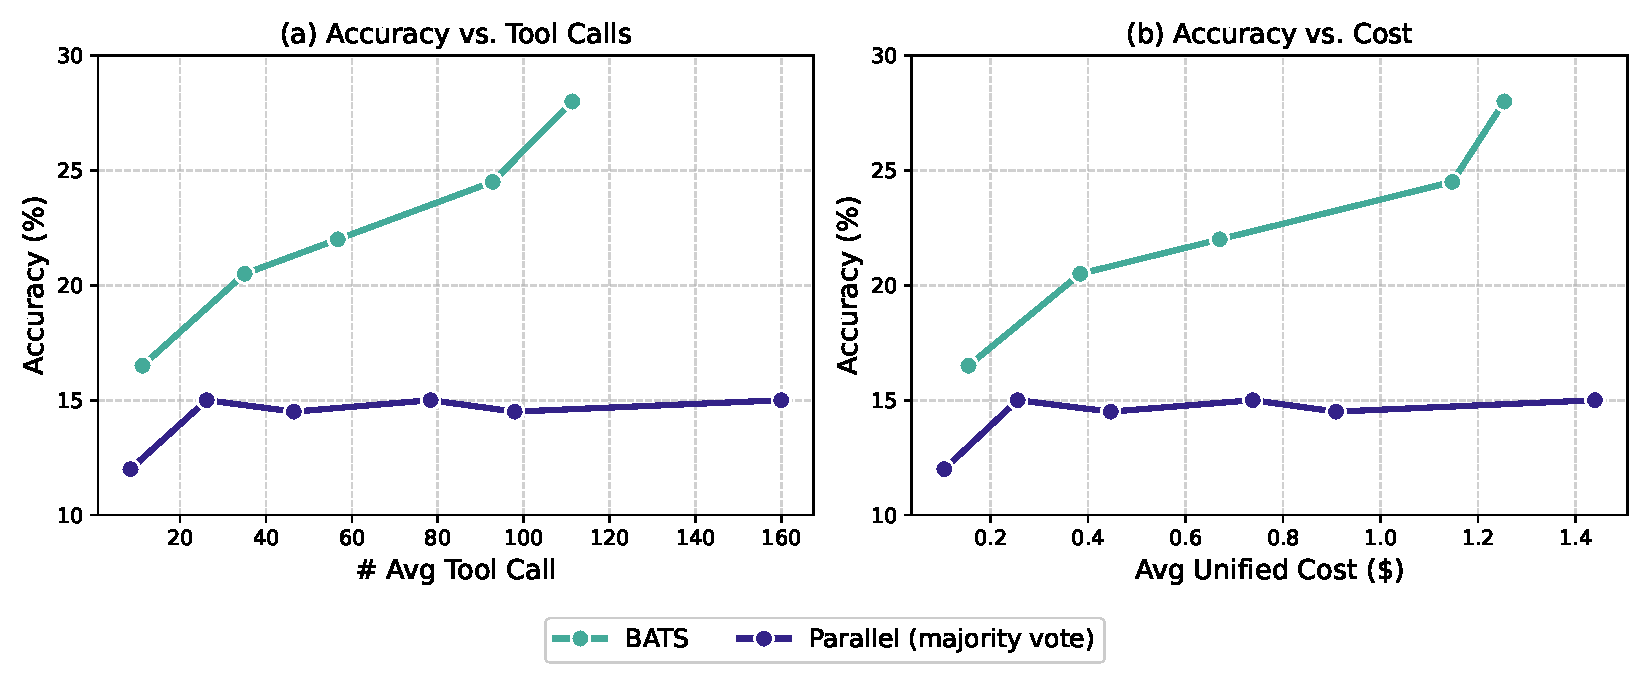
\includegraphics[width=0.9\linewidth]{assets/figs/bats_scaling_combined.pdf}
    \caption{Scaling behaviors along (a) total number of tool calls and (b) average unified cost, evaluated on a 200-example subset of BrowseComp using Gemini-2.5-Pro.}
    \label{fig:two}
\end{figure}


\textbf{\method achieves higher performance under the same budget constraint.} To better understand the scaling behavior, we vary the tool-call budget and evaluate performance on a random subset of 200 examples from BrowseComp for a manageable analysis.
Figure~\ref{fig:two} (left) shows the accuracy against the average number of tool calls, including both search and browse.
Across all budget levels, \method consistently outperforms the parallel majority-vote baseline, demonstrating that budget-aware adaptation leads to more effective use of limited tool calls.

\textbf{\method achieves higher performance when accounting for unified costs.}
Beyond tool-call counts, we measure performance under a unified cost metric that incorporates both token usage and tool-call expenses. As shown in Figure~\ref{fig:two} (right), \method achieves more favorable scaling curves, delivering higher accuracy at comparable or lower costs. This indicates that \method not only improves effectiveness under budget constraints but also yields better cost–performance trade-offs.

\subsection{Early Stopping}

We analyze how effectively agents can solve questions under budget constraints when allowed to stop early, without exhausting all tool calls. This setting reflects realistic scenarios where efficient, confident answers are preferable to prolonged exploration.
To isolate this behavior, we focus on the agent’s \textit{first attempt} only. For \method, this is the first answer that successfully passes self-verification. For baselines that lack verification, we use the output from a single generation pass as their first attempt.
If any tool budget is exhausted before this first attempt completes, the agent will stop and output a final answer based on its progress so far. This evaluation captures both efficiency and robustness, testing whether agents can solve questions quickly without being forced to use their full budgets.


\begin{figure}[htbp]
    \centering
    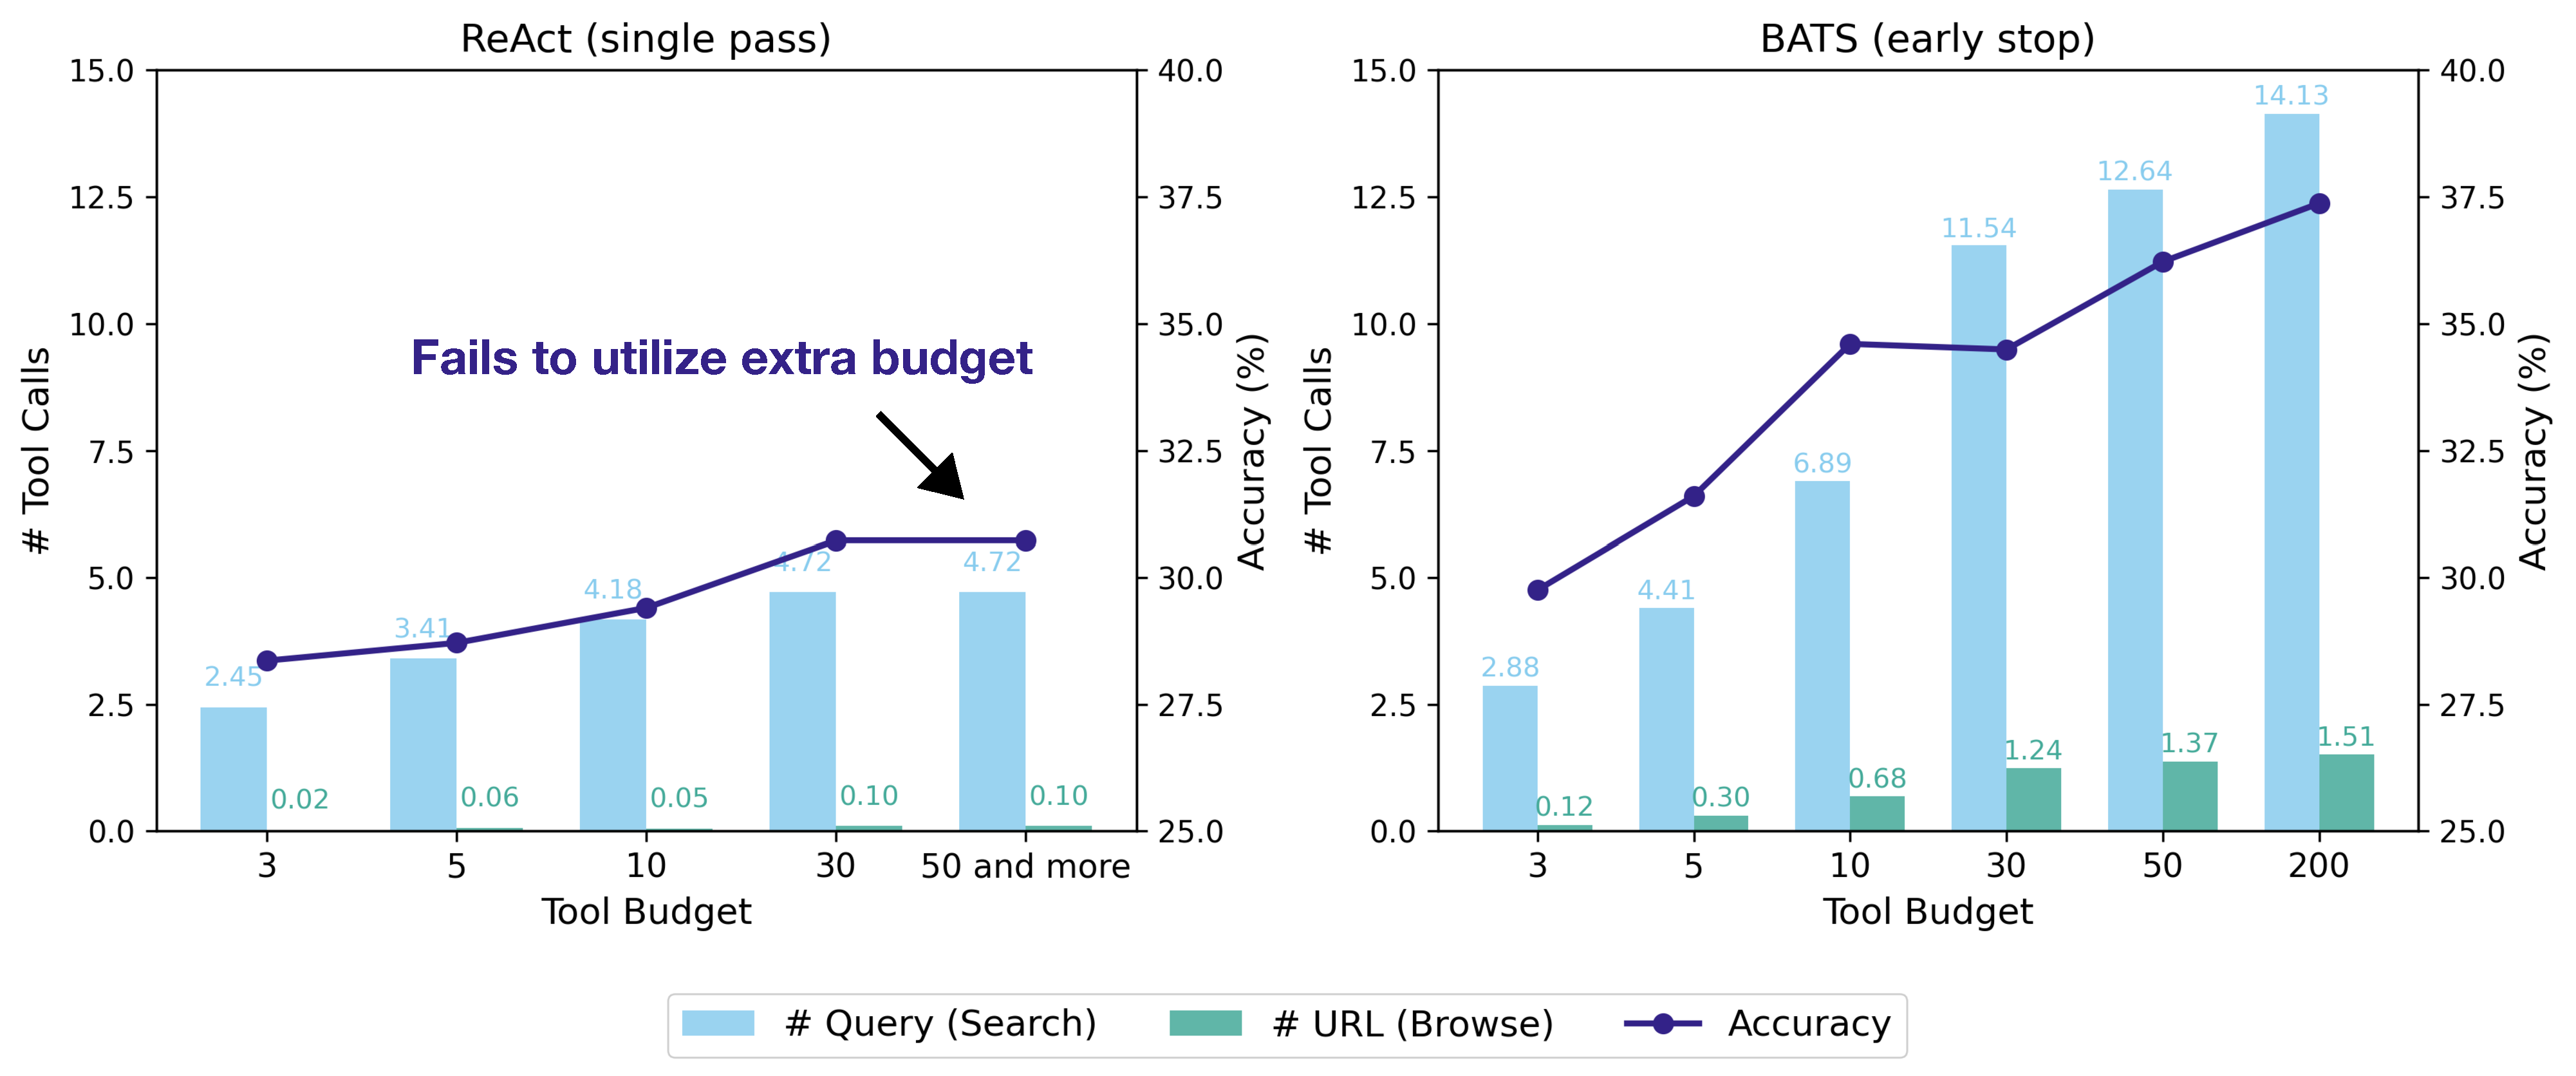
\includegraphics[width=0.95\linewidth]{assets/figs/early_stop_bczh_pro.pdf}
    \caption{Performance and resource utilization under early stopping on BrowseComp-ZH using Gemini-2.5-Pro. The bars represent the average number of Search and Browse tool calls (left axis), while the line plots indicate accuracy (right axis). While ReAct plateaus and fails to utilize additional budget, \method effectively scales up tool usage to achieve higher accuracy as the budget increases.}
    \label{fig:first-bczh}
\end{figure}




\textbf{Budget awareness enables \method to scale effectively with increased resources.} Figure~\ref{fig:first-bczh} presents the early stopping performance on BrowseComp-ZH using Gemini-2.5-Pro. The x-axis denotes the predefined tool call budget for both search and browse tool calls. Bars show the average number of tool calls actually used, while the line plot reports the resulting accuracy.
The ReAct baseline (Figure~\ref{fig:first-bczh} left) exhibits poor budget utilization: it consistently underuses the browse tool (fewer than 0.1 calls on average) and reaches a performance plateau early, with accuracy capped at 30.7\% for all budgets of 30 and above. This behavior highlights its lack of budget awareness and its inability to benefit from additional resources.
In contrast, \method (Figure~\ref{fig:first-bczh} right) shows strong budget-adaptive behavior. As the budget increases, it strategically raises its use of both search and browse tools, leading to steady gains in accuracy, rising from 29.8\% (budget=3) to 37.4\% (budget=200). 
Notably, with a budget of just 5, \method already surpasses the baseline’s best achievable accuracy. This demonstrates \method's ability to make more strategic and cost-effective decisions, delivering higher accuracy even with the same or fewer resources. More analysis can be found in Appendix~\ref{app:early}.



\subsection{Ablations}

\begin{table}[h]
\centering
\caption{Ablation results of BATS on three benchmarks with Gemini-2.5-Pro. The agent is provided a budget of 100 tool uses per tool. Removing different modules leads to various performance drops across datasets.}
\label{tab:ablations}
\begin{tabular}{lrrr}
\toprule
\textbf{Method} & \textbf{BrowseComp} & \textbf{BrowseComp-ZH} & \textbf{HLE-Search} \\
\midrule
BATS             & \textbf{18.7} & \textbf{39.1} & \textbf{23.0} \\
\quad w/o Planning     & 17.0 & 34.6 & 20.0 \\
\quad w/o Verification & 15.4 & 37.7 & 22.0 \\
\quad w/o Planning \& Verification  & 14.6  & 32.9   & 21.5 \\
\bottomrule
\end{tabular}
\end{table}


In this section, we present an ablation analysis of the key modules within \method using Gemini-2.5-Pro. The full comparison is shown in Table~\ref{tab:ablations}. Across all settings and datasets, the agent is allocated a budget of 100 tool uses per tool. To provide a clearer view of the orchestration framework, we focus on \method under the early-stopping mechanism, where generation terminates once an answer is verified as successful.

Results indicate that removing the planning module leads to a moderate performance decrease. However, removing the verification module causes a more significant drop on BrowseComp (from 18.7\% to 15.4\%). This suggests that the verification module is crucial for enabling the agent to navigate the solution space and accurately assess its current progress. Removing both modules results in lower performance (14.6\% on BrowseComp), while BrowseComp-ZH and HLE-Search exhibit some variance, likely due to the smaller dataset size. In addition, questions in HLE-Search are typically shorter and contain fewer details that can be verified, which limits the contribution of the verification module. Overall, the trend confirms that both modules contribute positively to the orchestration framework's effectiveness.

